\chapter{Multi-Scale Variance Stabilizing Transform on the Sphere (MS-VSTS)}
\label{ch_msvsts}

% \markright{Multi-Scale Variance Stabilizing Transform on the Sphere (MS-VSTS)}

\section{Principle of VST}

\subsection{VST of a Poisson process}

Given Poisson data $\mathbf{Y} := (Y_i)_i$, each sample $Y_i \sim \mathcal{P} (\lambda_i)$ has a variance $\text{Var}[Y_i] = \lambda_i$. Thus, the variance of $\mathbf{Y}$ is signal-dependant. The aim of a VST $\mathbf{ T}$ is to stabilize the data such that each coefficient of $\mathbf{ T}(\mathbf{Y})$ has an (asymptotically) constant variance, say $1$, irrespective of the value of $\lambda_i$. In addition, for the VST used in this study, $T(\mathbf{Y})$ is asymptotically normally distributed. Thus, the VST-transformed data are asymptotically stationary and gaussian.

The Anscombe transform \citep{rest:anscombe48} is a widely used VST which has a simple square-root form
\begin{equation}
\label{eq14}
\mathbf{ T}(Y):=2\sqrt{Y+3/8}.
\end{equation}
We can show that $\mathbf{ T}(Y)$ is asymptotically normal as the intensity increases.
\begin{equation}
\label{eq15}
\mathbf{ T}(Y)-2\sqrt{\lambda} \autorightarrow{$\mathcal{D}$}{$\lambda \rightarrow + \infty$} \mathcal{N}(0,1)
\end{equation}
It can be shown that the Anscombe VST requires a high underlying intensity to well stabilize the data (typically for $\lambda \geqslant 10$) \citep{starck:zhang07}.

\subsection{VST of a filtered Poisson process}

Let $Z_j := \sum_i h[i] Y_{j-i}$ be the filtered process obtained by convolving $(Y_i)_i$ with a discrete filter $h$. We will use $Z$ to denote any of the $Z_j$'s. Let us define $\tau_k := \sum_i (h[i])^k$ for $k=1,2,\cdots$. In addition, we adopt a local homogeneity assumption stating that $\lambda_{j-i} = \lambda$ for all $i$ within the support of $h$.

We define the square-root transform $T$ as follows:
\begin{equation}
\label{eq16}
T(Z):=b\cdot \mathrm{sign}(Z+c) |Z+c|^{1/2},
\end{equation}
where $b$ is a normalizing factor.  \\
\emph{\textbf{(Square root as VST)}} If $\tau_1 \neq 0$, $\|h\|_2,\|h\|_3<\infty$, then we have : \\
\begin{equation} \label{eq17}
\begin{split}
\mathrm{sign}(Z+c)\sqrt{|Z+c|}-\mathrm{sign}(\tau_1)\sqrt{|\tau_1|\lambda} \\
 \autorightarrow{$\mathcal{D}$}{$\lambda \rightarrow + \infty$} \mathcal{N}\Big(0,\frac{\tau_2}{4|\tau_1|}\Big).
\end{split}
\end{equation}
This  proves that $T$ is a VST for a filtered Poisson process (with a nonzero-mean filter) in that $T(Y)$ is asymptotically normally distributed with a stabilized variance as $\lambda$ becomes large (see \citet{starck:zhang07} for a proof).


\section{MS-VSTS}


The MS-VSTS~\citep{Schmitt} consists in combining the square-root VST with a multi-scale transform on the sphere.

\subsection{MS-VSTS + IUWT}

This section describes the MS-VSTS + IUWT, which is a combination of a square-root VST with the IUWT. The recursive scheme is:
\begin{equation}
\label{eq27}
\begin{split}
&\text{IUWT}\left\{\begin{array}{ccc}a_j  & = &  h_{j-1} \ast a_{j-1}  \\d_j  & = & a_{j-1}  - a_j  \end{array}\right. \\
 \Longrightarrow & \begin{split}\text{MS-VSTS} \\  \text{+ IUWT} \end{split}\left\{\begin{array}{ccc}a_j  & = &  h_{j-1} \ast a_{j-1} \\d_j  & = & T_{j-1}(a_{j-1}) - T_j(a_j) \end{array}\right. .
\end{split}
\end{equation}

In (\ref{eq27}), the filtering on $a_{j-1}$ can be rewritten as a filtering on $a_0 := \mathbf{Y}$, i.e., $a_j = h^{(j)} \ast a_0$, where $h^{(j)} = h_{j-1} \ast \cdots \ast h_{1} \ast h_0$ for $j \geqslant 1$ and $h^{(0)} = \delta$, where $\delta$ is the Dirac pulse ($\delta = 1$ on a single pixel and $0$ everywhere else). $T_j$ is the VST operator at scale $j$:
\begin{equation}
\label{eq28}
T_j(a_j) = b^{(j)} \mathrm{sign}(a_j+c^{(j)})\sqrt{|a_j + c^{(j)}|} .
\end{equation}
Let us define $\tau_k^{(j)}:=\sum_i (h^{(j)}[i])^k$. In~\citet{starck:zhang07}, it has ben shown that, to have an optimal convergence rate for the VST, the constant $c^{(j)}$ associated to $h^{(j)}$ should be set to:
\begin{equation}
\label{eq29}
c^{(j)}:=\frac{7\tau_2^{(j)}}{8\tau_1^{(j)}} - \frac{\tau_3^{(j)}}{2\tau_2^{(j)}} .
\end{equation}
The MS-VSTS+IUWT procedure is directly invertible as we have:
\begin{equation}
\label{eq30}
a_0 (\theta,\varphi) = T_0^{-1} \Bigg[ T_J(a_J) + \sum_{j=1}^J d_j \Bigg] (\theta,\varphi).
\end{equation}
Setting $b^{(j)}:=\text{sgn}(\tau_1^{(j)})/\sqrt{|\tau_1^{(j)}|}$, if $\lambda$ is constant within the support of the filter.
$h^{(j)}$, then we have \citep{starck:zhang07}:
\begin{equation}
\label{eq31}
\begin{split}
d_j(\theta,\varphi) \autorightarrow{$\mathcal{D}$}{$\lambda \rightarrow + \infty$} 
\mathcal{N} \Bigg( 0 , \frac{\tau_2^{(j-1)}}{4\tau_1^{(j-1)^2}} +\\ \frac{\tau_2^{(j)}}{4\tau_1^{(j)^2}} - \frac{\langle h^{(j-1)},h^{(j)} \rangle}{2\tau_1^{(j-1)}\tau_1^{(j)}} \Bigg) ,
\end{split}
\end{equation}
where $\langle . , . \rangle$ denotes inner product.

It means that the detail coefficients issued from locally homogeneous parts of the signal follow asymptotically a central normal distribution with an intensity-independant variance which relies solely on the filter $h$ and the current scale for a given filter $h$. Consequently, the stabilized variances and the constants $b^{(j)}$,$c^{(j)}$,$\tau_k^{(j)}$ can all be pre-computed.
Let us define $\sigma_{(j)}^2$ the stabilized variance at scale $j$ for a locally homogeneous part of the signal:
\begin{equation}
\label{eq32}
\sigma_{(j)}^2 = \frac{\tau_2^{(j-1)}}{4\tau_1^{(j-1)^2}} + \frac{\tau_2^{(j)}}{4\tau_1^{(j)^2}} - \frac{\langle h^{(j-1)},h^{(j)} \rangle}{2\tau_1^{(j-1)}\tau_1^{(j)}} .
\end{equation}

To compute the $\sigma_{(j)}$, $b^{(j)}$,$c^{(j)}$,$\tau_k^{(j)}$, we only have to know the filters $h^{(j)}$. We compute these filters thanks to the formula $a_j = h^{(j)} \ast a_0$, by applying the IUWT to a Dirac pulse $a_0 = \delta$. Then, the $h^{(j)}$ are the scaling coefficients of the IUWT. The $\sigma_{(j)}$ have been precomputed for a 6-scaled IUWT (Table~\ref{sigmaj}). 

\begin{table*}[!h]
  \centering
    \caption{Precomputed values of the variances $\sigma_j$ of the wavelet coefficients.
  }
  \begin{tabular}{|c|c|}
\hline
Wavelet scale $j$ & Value of $\sigma_j$ \\
\hline
  1 & 0.484704 \\
  2 & 0.0552595 \\
  3 & 0.0236458 \\
  4 & 0.0114056 \\
  5 & 0.00567026 \\
\hline
\end{tabular}

  \label{sigmaj}
\end{table*}

We have simulated Poisson images of different constant intensities $\lambda$, computed the IUWT with MS-VSTS on each image and observed the variation of the normalized value of $\sigma_{(j)}$ ($\mathbf{ (\sigma_{(j)})_{\text{simulated}}} / (\sigma_{(j)})_{\text{theoretical}}$) as a function of $\lambda$ for each scale $j$ (Fig. \ref{sigma}). We see that the wavelet coefficients are stabilized when $\lambda \gtrsim 0.1$ except for the first wavelet scale, which is mostly constituted of noise. On Fig. \ref{ansc}, we compare the result of MS-VSTS with Anscombe + wavelet shrinkage, on sources of varying intensities. We see that MS-VSTS works well on sources of very low intensities, whereas Anscombe doesn't work when the intensity is too low.

\begin{figure}[htb]
\centering{
\hbox{
%\psfig{figure=sigma1.ps,widtht=2.9in}
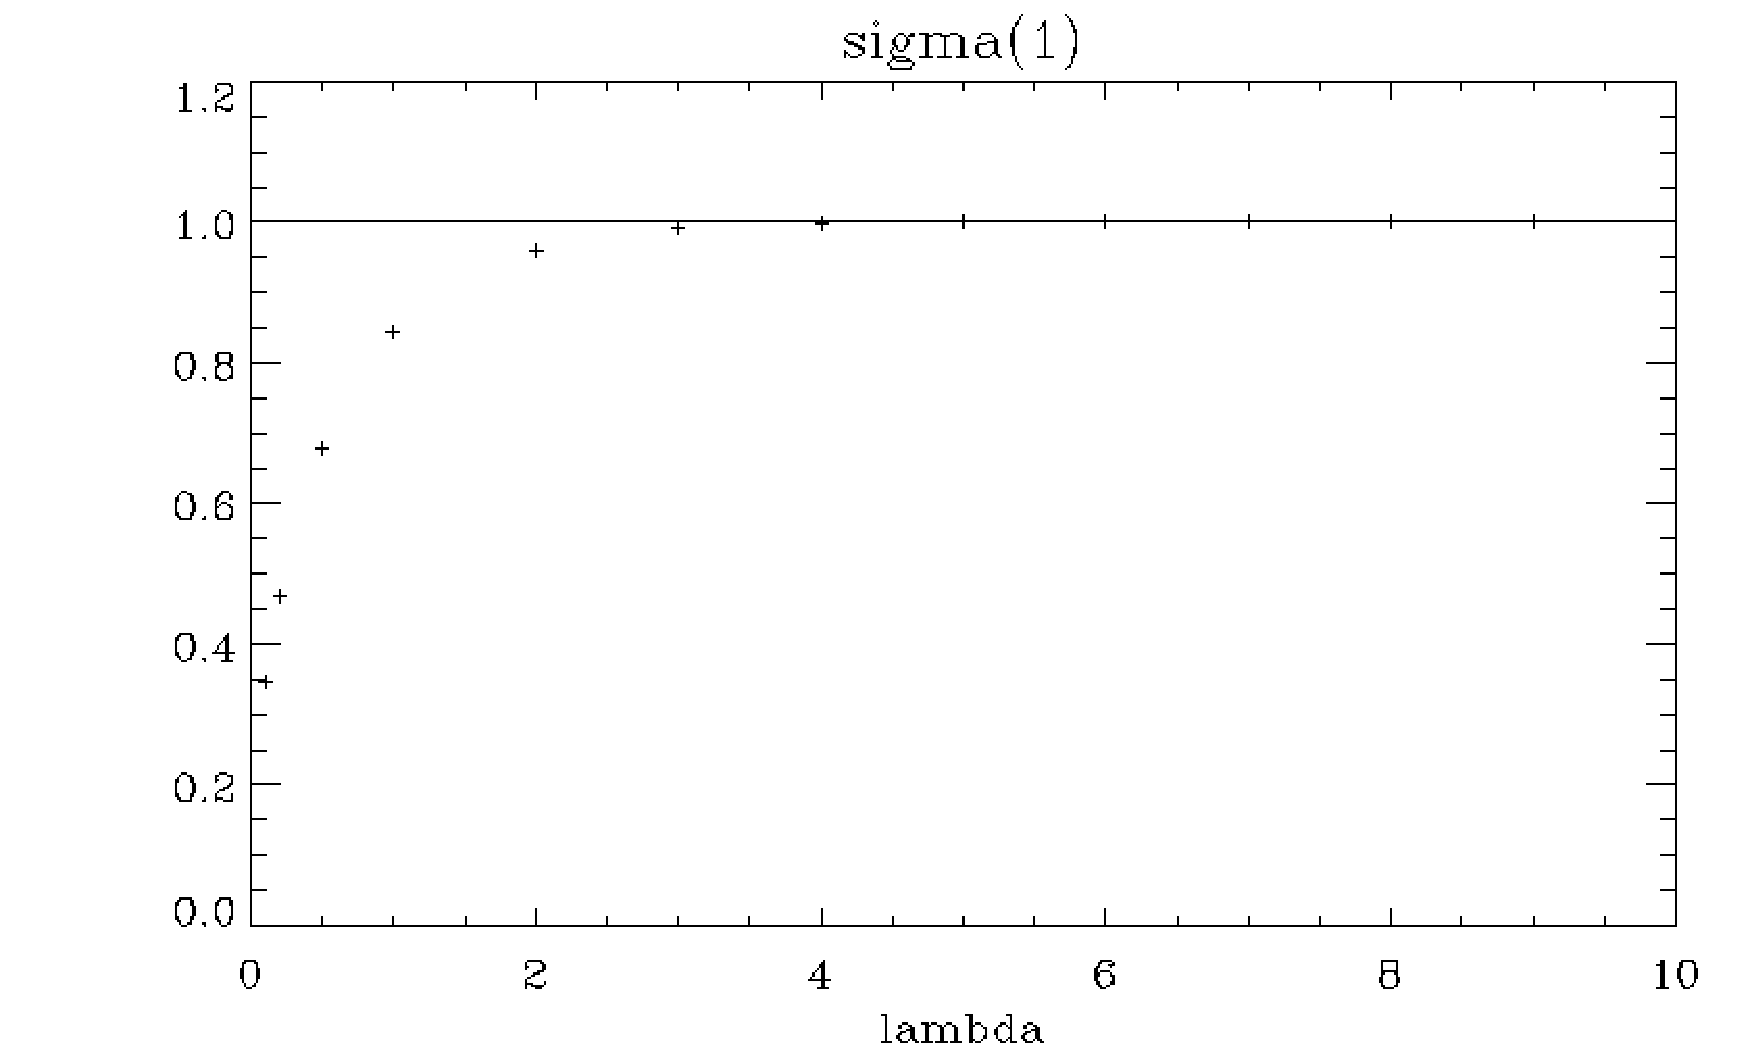
\includegraphics[width=2.5in, height=3in]{13822fg1.pdf}
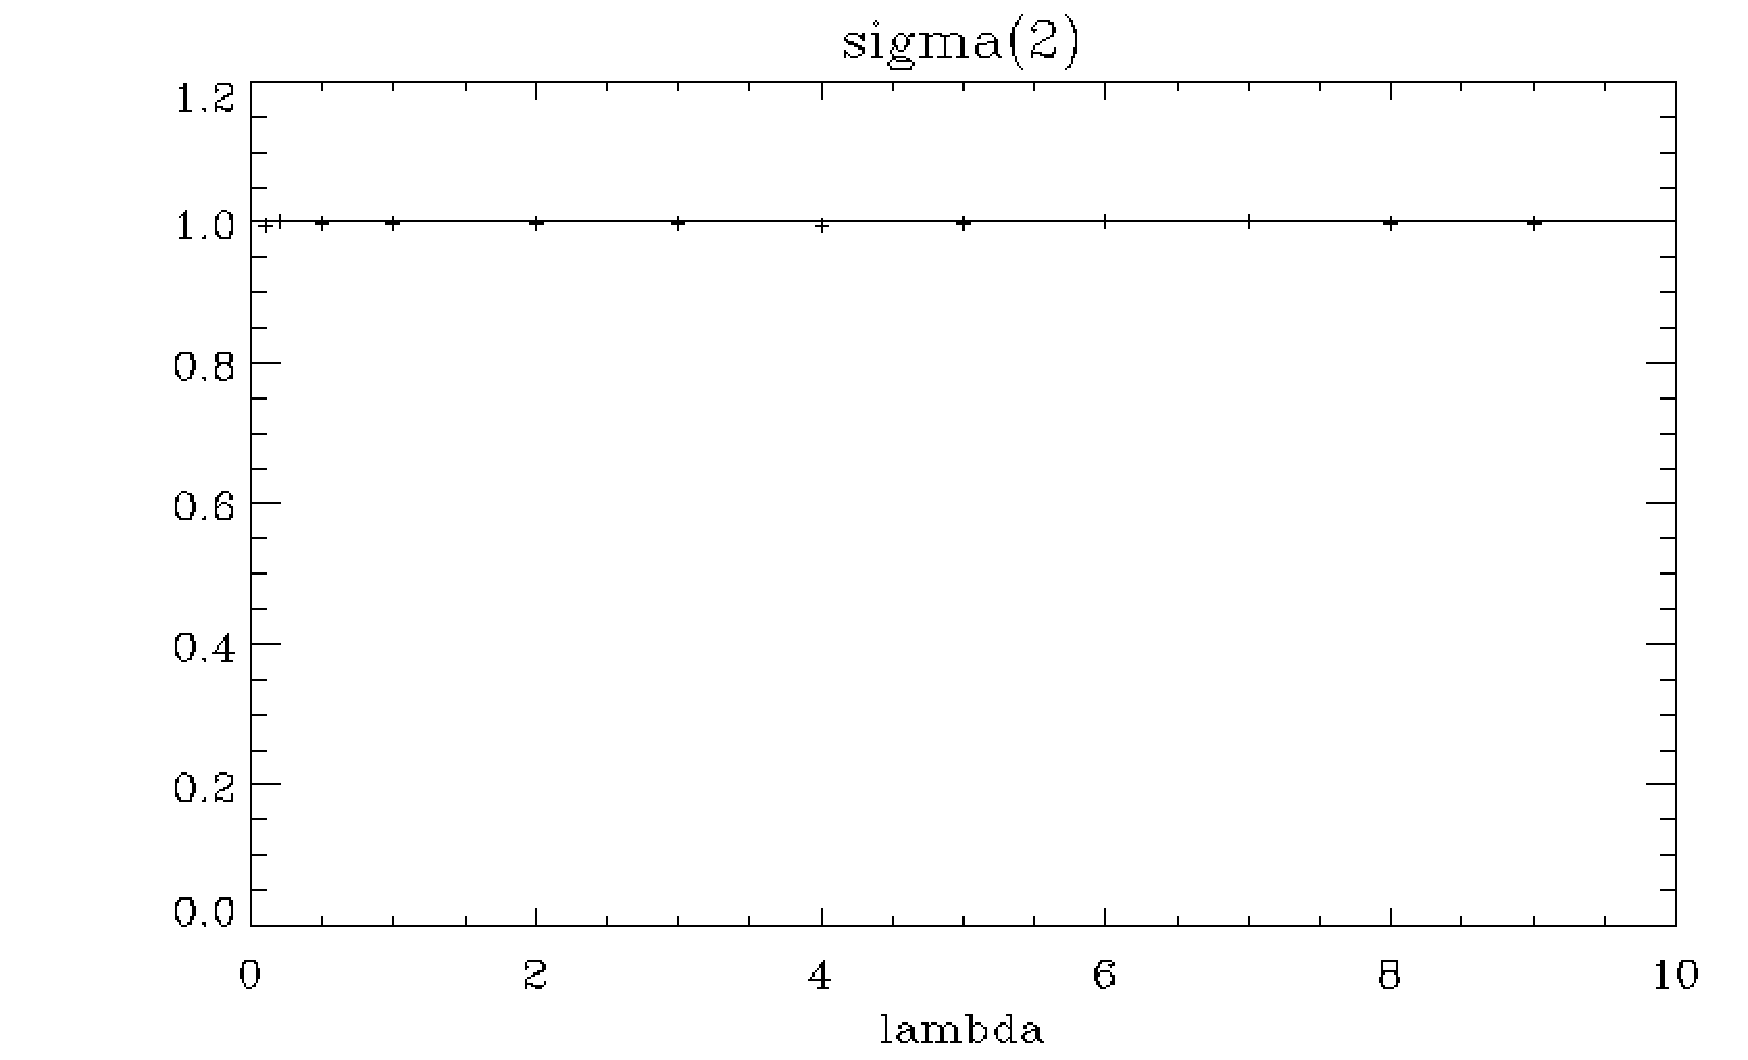
\includegraphics[width=2.5in, height=3in]{13822fg2.pdf}
}
\hbox{
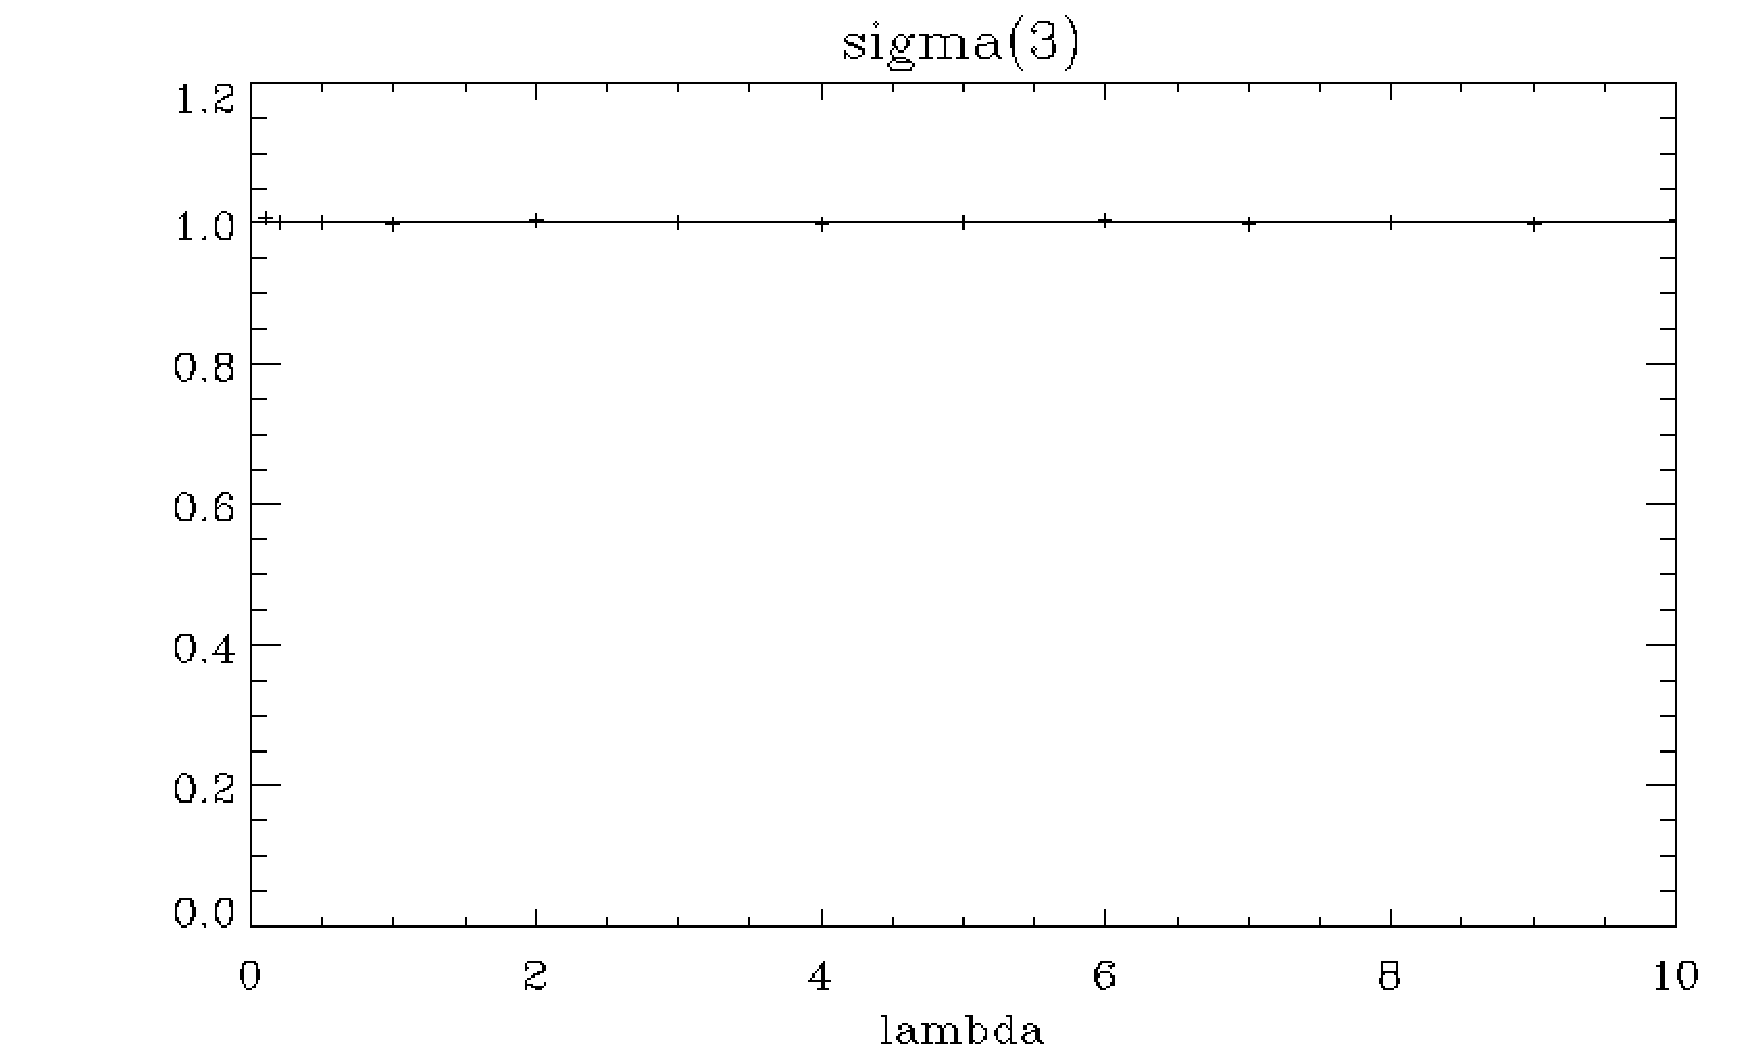
\includegraphics[width=2.5in, height=3in]{13822fg3.pdf}
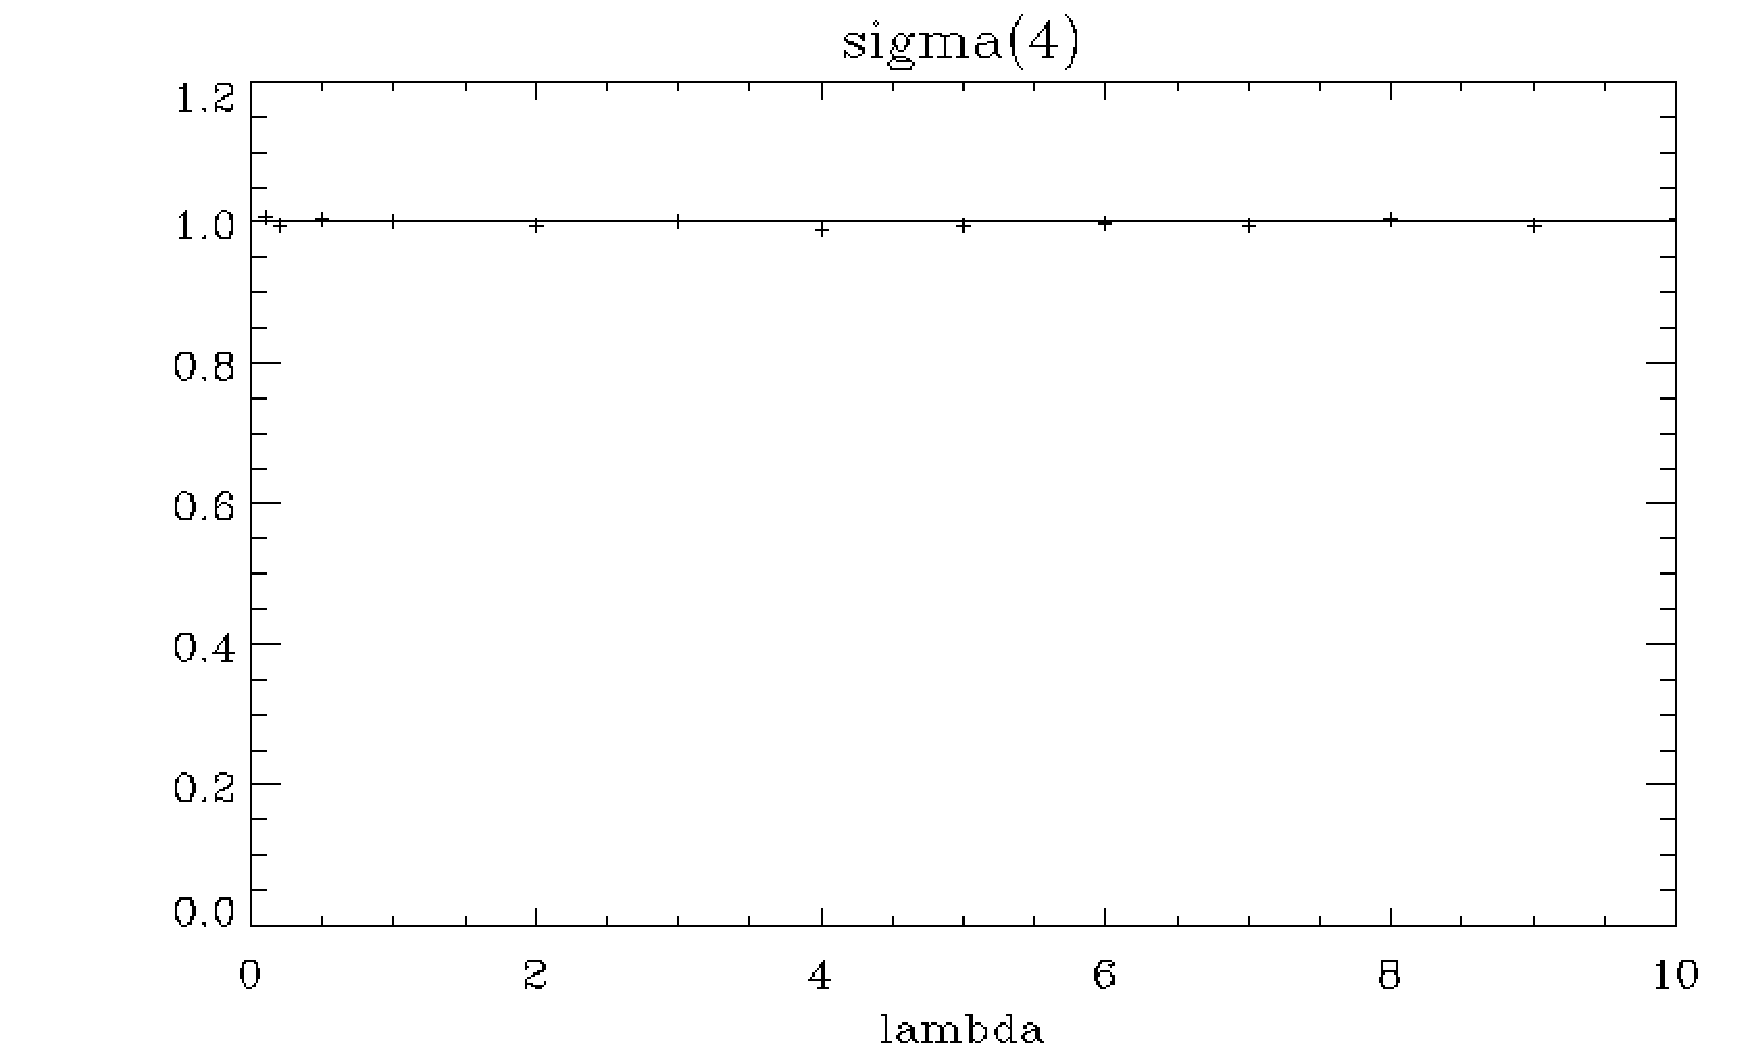
\includegraphics[width=2.5in, height=3in]{13822fg4.pdf}
}}
\caption{Normalized value ($\mathbf{ (\sigma_{(j)})_{\text{simulated}} }/ (\sigma_{(j)})_{\text{theoretical}}$) of the stabilized variances at each scale $j$ as a function of $\lambda$.}
\label{sigma}
\end{figure}

\begin{figure}[htb]
\centering
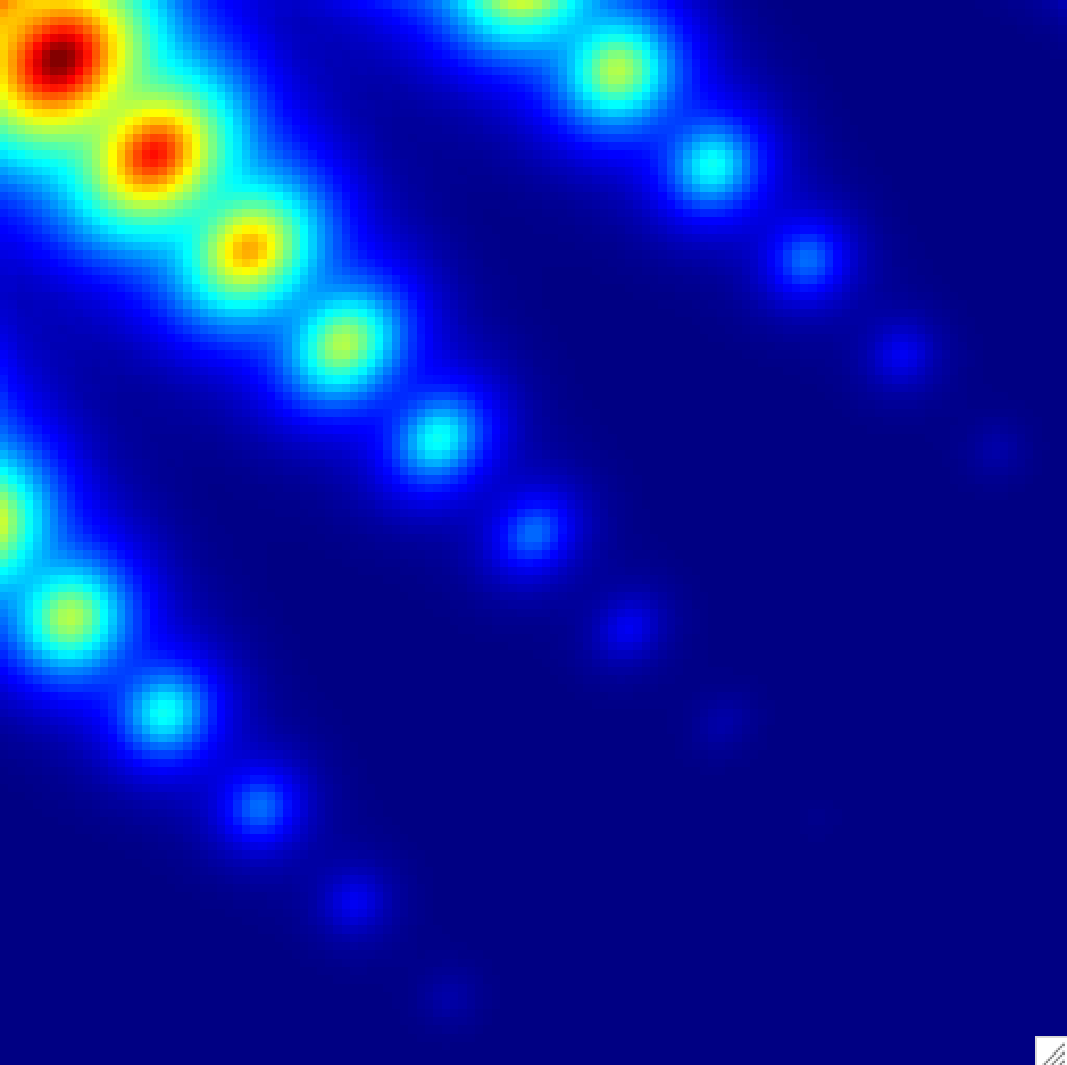
\includegraphics[width=2.5in]{13822fg6.pdf}
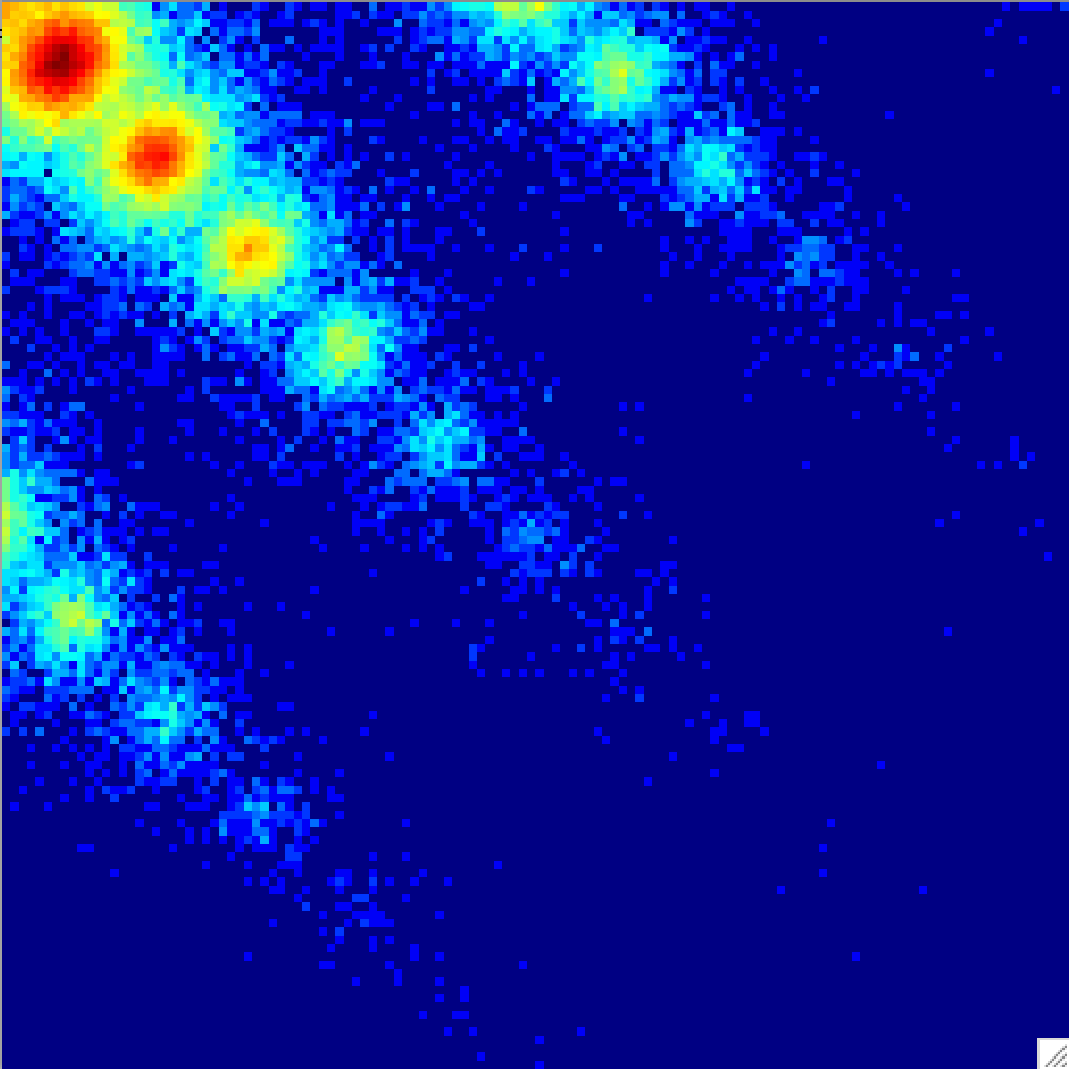
\includegraphics[width=2.5in]{13822fg7.pdf}
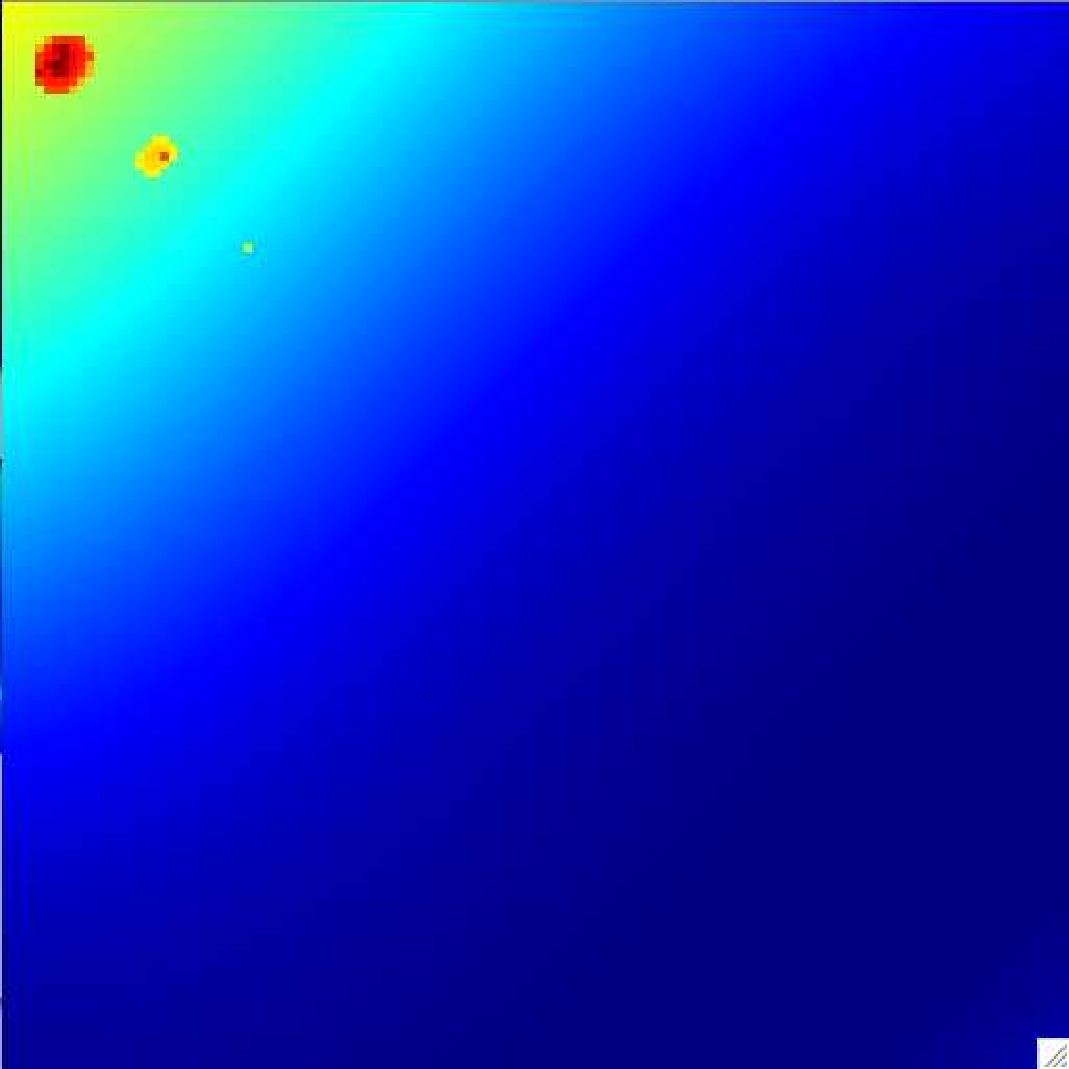
\includegraphics[width=2.5in]{13822fg8.pdf}
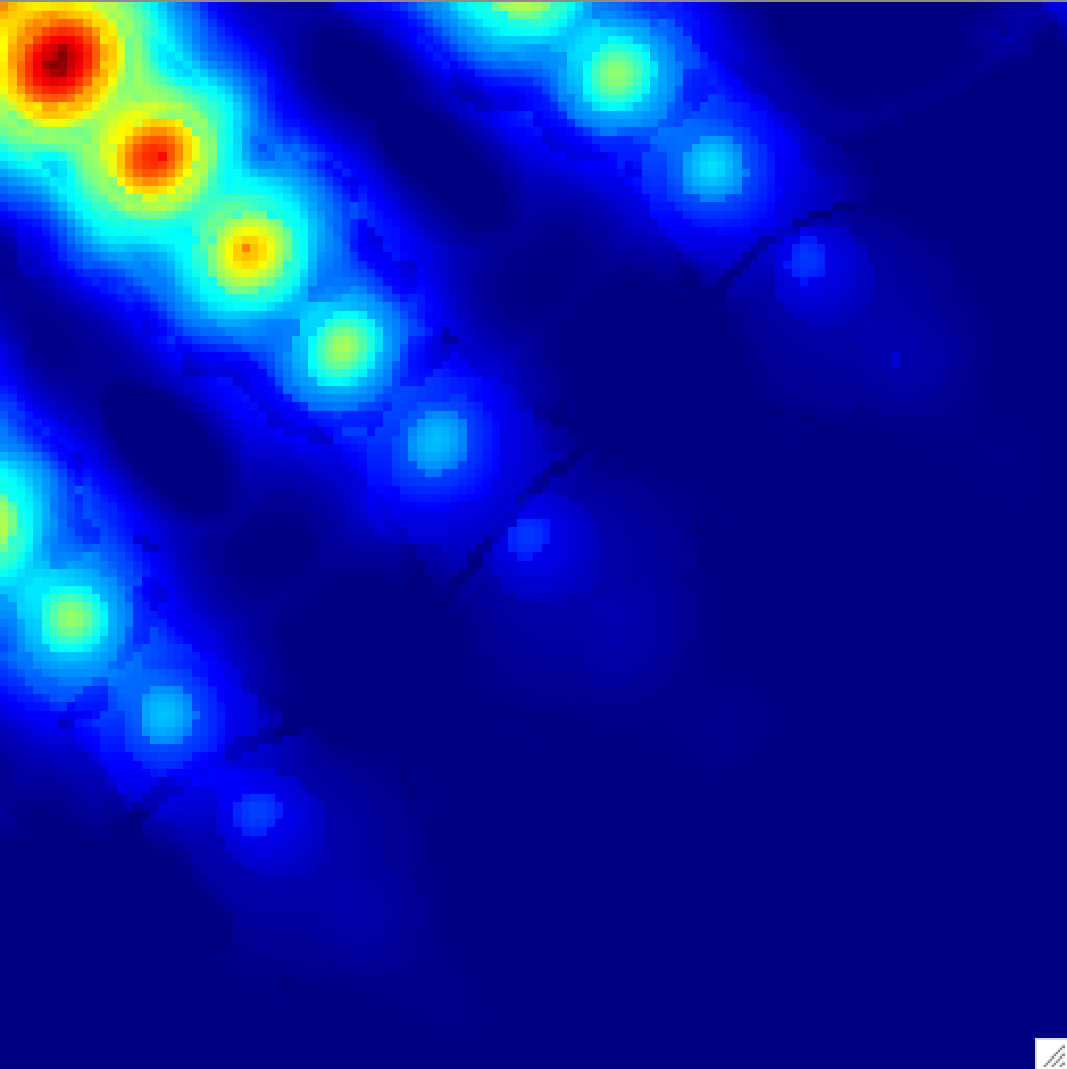
\includegraphics[width=2.5in]{13822fg9.pdf}
\caption{Comparison of MS-VSTS with Anscombe + wavelet shrinkage on a single HEALPix face.
\emph{Top Left} : Sources of varying intensity.
\emph{Top Right} : Sources of varying intensity with Poisson noise.
\emph{Bottom Left} : Poisson sources of varying intensity reconstructed with Anscombe + wavelet shrinkage.
\emph{Bottom Right} : Poisson sources of varying intensity reconstructed with MS-VSTS.
}
\label{ansc}
\end{figure}

\subsection{MS-VSTS + Curvelets}

As the first step of the algorithm is an IUWT, we can stabilize each resolution level as in Equation~(\ref{eq27}). We then apply the local ridgelet transform on each stabilized wavelet band.

It is not as straightforward as with the IUWT to derive the asymptotic noise variance in the stabilized curvelet domain. In our experiments, we derived them using simulated Poisson data of stationary intensity level $\lambda$. After having checked that the standard deviation in the curvelet bands becomes stabilized as the intensity level increases (which means that the stabilization is working properly), we stored the standard deviation $\sigma_{j,l}$ for each wavelet scale $j$ and each ridgelet band $l$ (Table~\ref{tabcurv}).

\begin{table*}[!h]
  \centering
   \caption{Asymptotic values of the variances $\sigma_{j,k}$ of the curvelet coefficients.
  }
  \begin{tabular}{|c|c|c|c|c|}
\hline
 $j$ & $l=1$ & $l=2$ & $l=3$ & $l=4$ \\
\hline
  1 & 1.74550 & 0.348175 & & \\
  2 & 0.230621 & 0.248233 & 0.196981 & \\
  3 & 0.0548140 & 0.0989918 & 0.219056 & \\
  4 & 0.0212912 & 0.0417454 & 0.0875663 & 0.20375 \\
  5 & 0.00989616 & 0.0158273 & 0.0352021 & 0.163248 \\
\hline
\end{tabular}
 
  \label{tabcurv}
\end{table*}
